% \section{Methods}
\noindent

This section details the goal, research questions, and the approach, including setup, and metrics used to rigorously test and validate our proposed method.

\begin{figure*}
\centering
%\noindent
% \centerline{\includegraphics[width=\textwidth]{images/FSE_RefRL_overview_cropped.pdf}}
\centerline{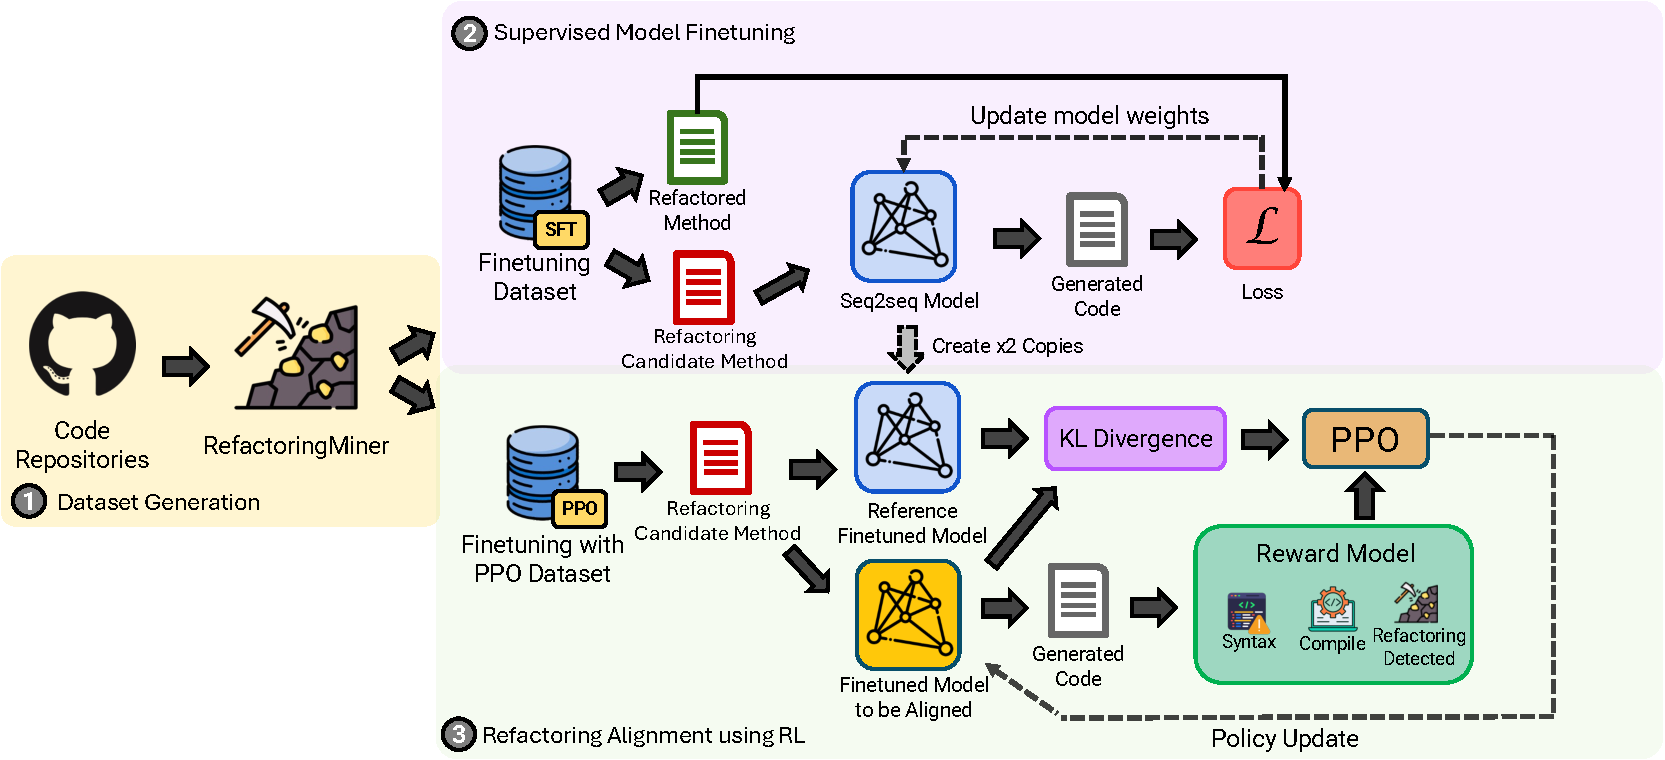
\includegraphics[width=\textwidth]{chapters/generation/images/overview_cropped.pdf}}
\caption{Overview of the proposed approach.}
\label{fig:methodology}
% \vspace{-5pt}
\end{figure*}

\subsection{Overview}
% \todo{Please follow goal -> RQs -> approach}

The goal of this study is to evaluate the effectiveness of fine-tuned \llmsc{}s pretrained on code and develop a deep reinforcement learning-based approach for generating code for extract method refactoring. We seek to demonstrate the effectiveness of our approach not only quantitatively but also qualitatively.
% This study proposes an approach to fine-tune a \LLM{} (LLM) using deep reinforcement learning for automatically generating extracted methods and modified original methods after performing \exm{} refactoring. 
We formulate the following research questions.
\newpage
\begin{description}

    \item [\textbf{RQ1.}] \textit{How does supervised fine-tuning perform for extract method refactoring task?}


By answering this research question, we aim to evaluate how well does supervised fine-tuning a code \llm{} perform in automatically performing \exm{} refactoring.


    % \item [\textbf{RQ2.}] \textit{How accurately a reinforcement learning approach performs for automating \exm{} refactoring?}
    \item [\textbf{RQ2.}] \textit{How well does a reinforcement learning approach perform for automating extract method refactoring?}


% This research question aims to assess whether \llm{}s pre-trained on code can be \textbf{directly} aligned using a reinforcement learning technique to perform \exm{} refactoring task effectively.
This question examines whether code \llm{}s can be directly aligned using reinforcement learning techniques to effectively perform \exm{} refactoring.


    % \item [\textbf{RQ3.}] \textit{How accurately a reinforcement learning approach aligned with fine-tuned \llmsc{} for code performs for automating \exm{} refactoring?}
    \item [\textbf{RQ3.}] \textit{How does a reinforcement learning approach, combined with fine-tuned \llm{}s, perform for automating extract method refactoring?}

This question assesses the impact of combining Proximal Policy Optimization (\ppo{}) with custom reward signals on a fine-tuned model's performance in \exm{} refactoring tasks.
\end{description}

Figure~\ref{fig:methodology} illustrates our methodology. We create our dataset by using the tools such as SEART tool~\cite{seart2021data} and RefactoringMiner~\cite{Tsantalis:TSE:2020:RefactoringMiner2.0, Tsantalis:ICSE:2018:RefactoringMiner}.
Following dataset preparation, we fine-tune four different models: \codetf{} and \plbart{}, which are encoder-decoder models, and \codegpt{} and \codegen{}, which are decoder-only models. We evaluate the performance of these models using both quantitative and qualitative measures. After conducting both quantitative and qualitative evaluations, we align the pre-trained model directly using the Proximal Policy Optimization (\ppo{}) algorithm. Subsequently, we align the fine-tuned model using the same \ppo{} algorithm.
We systematically evaluate the applied approach using standard evaluation metrics. We also evaluate the models qualitatively using three key checks \ie{} syntactic validity, compilability, and the presence of the desired refactoring in the generated code.

\subsection{Dataset Creation} \label{section:dataset_creation}

We employ a systematic approach to identify and collect extract method refactoring instances across multiple open-source Java repositories. Step~\circled{1} in Figure~\ref{fig:methodology} shows an overview of the dataset preparation pipeline. 
We use SEART~\cite{seart2021data} tool to select a  list of repositories for analysis. 
SEART tool is a GitHub project sampling tool,
offering various commonly used filters (such as number of commits and stars).
We obtain a list of all non-forked Java repositories 
created between $2013$ and $2023$, that are active in $2024$, 
have at
least $100$ commits,
and minimum $50$ stars. 
We obtained a total of $1,618$ repositories
satisfying the criteria.

\begin{algorithm}[th!]
\caption{Procedure for Creating Dataset}
\label{algo:1}
\begin{algorithmic}[1]
    \State \textbf{Input:} List of repositories $R = \{r_1, r_2, \dots, r.
    _n\}$
    \State \textbf{Output:} JSONL file with keys ``Input'' and ``Output''
    
    \Procedure{CreateDataset}{$R$}
        \State $Data \gets \emptyset$ \Comment{Initialize the dataset as an empty set}
        \For{each repository $r_i \in R$}
            \State Retrieve branch details for $r_i$
            \State Fetch the list of commits for the given branch
            \For{each commit $c_j$ in the list of commits}
                \State Identify refactorings performed in $c_j$
                \If{extract method refactoring is detected}
                    \State Extract metadata associated with the refactoring
                    \State Extract the refactored method using the metadata
                    \State Checkout to the previous commit $c_{j-1}$
                    \State Extract the original method from $c_{j-1}$
                    \State Create output JSON object 
                    \State Append this JSON object to $Data$
                \EndIf
            \EndFor
        \EndFor
        \State Store $Data$ in a JSONL file
    \EndProcedure

\end{algorithmic}
\end{algorithm}



To iteratively process the list of repositories to prepare the dataset, we created a custom Command Line Interface (CLI) tool. 
Algorithm~\ref{algo:1} provides a pseudocode of the functionality of the tool. 
% \todo{explain Algo 1} 
For each repository, we retrieve branch details and fetch the commit history. We then iterate through each commit, identifying any extract method refactorings performed using RefactoringMiner~\cite{Tsantalis:ICSE:2018:RefactoringMiner, Tsantalis:TSE:2020:RefactoringMiner2.0}. When such a refactoring is detected, the algorithm extracts relevant metadata and the refactored method from the current commit $c_j$. It then checks out the previous commit, $c_{j-1}$ to extract the original, pre-refactored method. This pair of pre- and post-refactoring methods, along with associated metadata (such as file path, class content and start and end line of the methods), is packaged into a JSON object. These JSON objects are accumulated into an array, which is ultimately stored in a JSONL file format. This approach enables the creation of a comprehensive dataset ($\mathcal{D}$) that captures the before and after states of extract method refactorings across multiple repositories.

% We iterate through this repository list, 
% passing the repository name and branch details to our CLI tool. 
% With the help of RefactoringMiner, the tool extracts the methods involved in \exm{} refactoring along with the associated metadata and stores all identified samples in \texttt{jsonl} file as json objects. 

\begin{table}[ht]
    \centering
    \caption{Dataset statistics} \label{tab:dataset_stats}
    \resizebox{\columnwidth}{!}{
        \begin{tabular}{ccc|ccc}
            \toprule
            \multirow{2}{*}{Dataset} & \multicolumn{2}{c}{Before pre-processing} & \multicolumn{2}{c}{After pre-processing} \\
            \cmidrule(lr){2-5}
& \makecell[c]{Avg.\\ source token\\ length} &  \makecell[c]{Avg. \\ target token\\ length} &  \makecell[c]{Avg.\\ source token\\ length} &  \makecell[c]{Avg.\\ target token\\ length} & \\
            \cmidrule(lr){1-5}
\makecell[l]{$\mathcal{D}_{SFT}$}& 412.77 & 446.13 & 184.26 & 241.63\\ \addlinespace
\makecell[l]{$\mathcal{D}_{RL}$} & 410.60 & 449.09 & 187.62 & 242.13 \\ \addlinespace
% \makecell[l]{$\mathcal{D}$} & 411.68 & 447.69 & 185.94 & 241.88 \\ 
            \bottomrule
        \end{tabular}    
    }
\end{table}
\vspace*{\fill}
% We applied the aforementioned procedure to process both  repository sets.
% \todo{change the acronym, as discussed.}
For RQ1 and RQ2, we use the entire dataset.
For RQ3,
we divide the dataset into two mutually exclusive subsets one for supervised fine tuning and the other for the aligning the fine-tuned model with deep reinforcement learning.
We divide the dataset to maintain data integrity and avoid data leak while training  for RQ3.
We divide the repository list of $1,618$ repositories, collected from the SEART tool, in half. We applied the aforementioned procedure to process both sets of repositories. This resulted in $38,441$ samples for the supervised fine tuning ($\mathcal{D}_{SFT}$) and $9,313$ samples for deep reinforcement learning ($\mathcal{D}_{RL}$).
However, the resulting datasets contained samples that exceeded the context window (maximum input sequence length) of our selected fine-tuning models.
Among these models, \texttt{Code-T5} has the smallest context window of $512$ tokens, while others support up to $2,048$ tokens. To ensure compatibility across all models, we use $512$ as our maximum context length, eliminating any samples that surpassed this $512$-token threshold. After pre processing, $\mathcal{D}_{SFT}$ contains $26,949$ samples and $6,528$ samples in $\mathcal{D}_{RL}$. 
Table~\ref{tab:dataset_stats} presents the average token length distribution for both the datasets. Finally, each of the dataset is divided in $70:20:10$ ratio for training, testing and validation.

\subsection{Training Models}



\subsubsection{Fine tuning LLMs}

% \todo{IP: Setup information}
We employ the following criteria to select the models for fine-tuning.
The selected models must belong to encoder-decoder or decoder-only architecture.
We exclude encoder-only models, such as CodeBERT, from our study because the encoder-only models are not well-suited for sequence-to-sequence (seq2seq) generation tasks~\cite{wang2023codet5+}.
% \todo{state any other criterion; like size? common used or should not be too big? - DONE}  
Encoder-only model architectures like \textsc{bert} are designed to understand input sequences but lack the ability to generate new ones. They're optimized for tasks like classification or feature extraction, not for producing variable-length outputs required in seq2seq tasks. Without a decoder component and autoregressive generation capability, these models can't effectively perform tasks such as translation or text generation that require producing new sequences based on input.
We select the following models, two belonging to encoder-decoder and two to decoder-only architecture family,
based on the the above-mentioned criteria.

\begin{itemize}
    \item \textbf{Code-T5}: \codetf{}~\cite{wang2021codet5identifierawareunifiedpretrained} is a pre-trained encoder-decoder model that incorporates token type information from code and employs an identifier-aware pre-training objective to better utilize identifiers. \codetf{} offers a unified framework that supports both code understanding and generation tasks, enabling multi-task learning. 
    This model has been successfully applied to various code related tasks such as code summarization~\cite{al2023extending, gu2022assemble}, code translation~\cite{kusum2022unsupervised} and vulnerability detection~\cite{paul2023, hou2024largelanguagemodelssoftware}.

    \item \textbf{PLBART}: \plbart{}~\cite{ahmad2021} 
    % \todo{structure references as <Last name><year> format}
    is a pre-trained sequence-to-sequence model that can perform a wide range of program and language understanding and generation tasks. It is trained on a large dataset of Java and Python functions along with their associated natural language text using denoising autoencoding. 
    \plbart{} has been used in various software engineering applications especially in program repair task~\cite{paul2023, wu2023effective}

    \item \textbf{CodeGPT-adapt}: \codegpt{}~\cite{lu2021codexgluemachinelearningbenchmark} is a GPT-2-based decoder-only Transformer model for code completion, pre-trained on Python and Java code from CodeSearchNet datasets. It learns code structure and syntax through pre-training, enabling it to generate code automatically.
    It has been widely used for code generation tasks such as code completion~\cite{li2024ircoco, hou2024largelanguagemodelssoftware}.

    \item \textbf{CodeGen}: \codegen{}~\cite{nijkamp2022codegen} is a Transformer-based autoregressive language model trained on natural language and programming language datasets. It employs next-token prediction as its learning objective and has shown outstanding performance in program synthesis tasks~\cite{christopoulou2022pangu}.

\end{itemize}

Step~\circled{2} in Figure~\ref{fig:methodology} illustrates the \textsc{sft} strategy employed for extract method refactoring. To train the encoder-decoder models, the pre-refactored code is first tokenized to serve as the input sequence. After a forward pass through the model, output tokens are generated and decoded using the same tokenizer. The resulting method is then compared to the ground truth, which includes both the extracted method and the modified original method post-refactoring. The model weights are updated based on the cross-entropy loss computed between the predicted and ground truth methods.

For decoder-only models, the training process is similar, with the key difference being in the format of the input. In this case, the input sequence is formed by concatenating the pre-refactored code and the ground truth output, separated by a special \textsc{[SEP]} token. This format enables the model to learn from both the context of the original code and the desired output sequence in a single input representation.


\subsubsection{Aligning the models with RL}

In this study, we fine-tune and align the selected \llm{}s for \exm{} refactoring using \rl{} techniques (step~\circled{3}). 
We model the code transformation problem as a Markov Decision Process (MDP).
We define the \textit{state} as the set of all possible code representations and the state transition function as appending the chosen refactored token to the current sequence.

Algorithm~\ref{algo:2} describes the pseudocode for aligning the fine tuned language model for extract method refactoring task. The algorithm starts with an initial policy (decision-making strategy) and a value function (which estimates how good a particular state is). It then goes through multiple training iterations to improve these over time. In each iteration, we sample a batch of code snippets from our \rl{} dataset. For each snippet, \textit{i.e.} the pre-refactored method, we use the current policy to generate a sequence of refactoring actions. To assess the quality of the sequence generated at each training step, we compute a reward based on three factors: syntactic correctness, compilation success, and whether the action is recognized as a valid refactoring. 


% \subsubsection*{Reward Modelling}

% We employ a carefully designed reward model to guide the reinforcement learning process. 
The reward function plays a crucial role in evaluating the quality and correctness of the refactoring suggestions produced by the model.
Our reward function consists of three key components, each addressing a specific aspect of the refactoring process:

\begin{enumerate}
    \item \textit{Syntactic Correctness:} We assess the presence of errors in the refactored code.
    For this purpose, we check the presence of error nodes in the Abstract Syntax Tree (\abst{}) generated by \textit{tree-sitter} of the generated code.
    \begin{equation} \label{eq:syntax}
        R_{syntax} = 
        \begin{cases}
            +1 & \text{if no error nodes} \\
            -1 & \text{if error nodes present}
        \end{cases}
    \end{equation}

    \item \textit{Compilation Success:} We verify whether the refactored code compiles successfully. While the compiler automatically checks for syntactic issues, separating syntactic correctness from compilation success allows us to provide the \rl{} model with more granular feedback. This distinction is important because refactored code might be syntactically correct but still fail to compile due to semantic errors.
    \begin{equation} \label{eq:compile}
        R_{compile} = 
        \begin{cases}
            +1 & \text{if code compiles} \\
            0 & \text{if code fails to compile}
        \end{cases}
    \end{equation}

    \item \textit{Refactoring Detection:} We validate the presence of extract method refactoring in the generated code using RefactoringMiner.
    \begin{equation} \label{eq: detect}
        R_{detect} = 
        \begin{cases}
            +1 & \text{if detected by RefactoringMiner} \\
            -1 & \text{if not detected}
        \end{cases}
    \end{equation}
\end{enumerate}

The sum of these individual components gives us the total reward for a given refactoring suggestion.

\begin{equation}
    R_{total} = R_{syntax} + R_{compile} + R_{detect}
\end{equation}

This reward function encourages the language model to generate syntactically correct, compilable code that successfully implements the extract method refactoring. 


The value head is used to estimate the value of the current state using the value function as shown in Equation~\ref{eq:value_func}. The algorithm then calculates how much better or worse each action was than expected (the \textit{advantage}). This information is used to update the policy, aiming to increase the probability of actions that led to high rewards. However, to ensure stable learning, the algorithm checks how much the new policy differs from the old one using a measure called KL divergence as described in equation~\ref{eq:kl_div}. If the difference is too large, the update is adjusted to prevent drastic changes. Finally, the value function is updated to better predict future rewards. By repeating this process many times, the algorithm gradually improves its ability to make good refactoring decisions. 


\begin{algorithm}
\caption{DRL Training for Extract Method Refactoring with KL Divergence}
\label{algo:2}
\begin{algorithmic}[1]
\Require Initial policy $\pi_\theta$, value function $V_\phi$, KL divergence coefficient $\beta$, weights $w_1, w_2, w_3$
\For{each training iteration}
\State Sample batch of code snippets from dataset
\For{each code snippet $x$}
\State Generate a refactored code snippet using current policy $\pi_\theta$
\State Compute syntactic correctness: $R_{syntax}$ using Eq.~\ref{eq:syntax}
\State Compute compilation success: $R_{compile}$ using Eq.~\ref{eq:compile}
\State Compute refactoring validity: $R_{detect}$ using Eq.~\ref{eq: detect}

\State Compute total reward: $R_{total} = w_1 \cdot R_{syntax} + w_2 \cdot R_{compile} + w_3 \cdot R_{detect}$
\State Estimate the value of the current state: $V_\phi(s)$
\State Calculate advantage: $A = R_{total} - V_\phi(s)$
\EndFor
\State Compute policy update to maximize:
\State \quad $J(\theta) = \mathbb{E}\left[\frac{\pi_{\theta}(a|s)}{\pi_{\theta_{old}}(a|s)} A\right] - \beta \cdot \text{KL}(\pi_{\theta_{old}} || \pi_{\theta})$
\State Apply the update to the policy: $\theta_{old} \leftarrow \theta$
\State Update value function to minimize: $L(\phi) = \sum (R_{total} - V_\phi(s))^2$
\EndFor
\end{algorithmic}
\end{algorithm}


\subsubsection{Fine tuning setup.} 

We fine-tune the supervised model for $10$ epochs on the dataset $\mathcal{D}$ for \textit{RQ1}, and on the dataset $\mathcal{D}_{SFT}$ 
for \textit{RQ3}. The training is conducted with a global batch size of $16$, using the Adam optimizer~\cite{kingma2017} with an initial learning rate of $1.33 \times 10^{-5}$. For aligning the models with \rl{}, we utilize and extend the \textsc{trl} Python library, which is widely used for training transformer language models with reinforcement learning. The generation parameters are set with \textit{min\_tokens} as $-1$ and \textit{max\_tokens} as $512$. The training consists of $20,000$ steps, with the model undergoing $10$ \ppo{} optimization epochs for each step. The code processes one batch per training step, generating responses, calculating rewards, and optimizing the model using PPO. For each batch, multiple internal PPO optimization passes are performed before moving to the next batch. This process repeats for $20,000$ steps, cycling through the dataset if necessary. A global batch size of $16$ is maintained, and the Adam optimizer~\cite{kingma2017} is employed. We apply Adaptive KL control with an initial KL coefficient of $0.2$. All experiments are conducted with a fixed seed value to ensure reproducibility and are performed on nodes of a High Performance Computing (HPC) cluster, utilizing $2$ V100-32GB GPUs and $32$ GB of RAM.

\subsection{Evaluation}
In this section, we summarize the metrics commonly used for code generation tasks.
Also, we provide details about qualitative evaluation that goes beyond the standard metrics.

\subsubsection{Evaluation Metrics}

To assess the effectiveness of our models quantitatively, we utilize established metrics from natural language processing field \bleu{}~\cite{papineni2002bleu} and \rouge{}~\cite{lin2004rouge}, as well as specialized metrics tailored for code evaluation, \codebleu{}~\cite{ren2020codebleumethodautomaticevaluation} and syntax match score~\cite{zhu2022xlcostbenchmarkdatasetcrosslingual}. 
The widespread adoption of these metrics in academic research for evaluating generative models supports our decision to use them. 


\subsubsection{Qualitative Evaluation} \label{subsubsection:qualitative}


To evaluate the effectiveness of our fine-tuned code language models in performing \exm{} refactoring, we construct a diverse test suite encompassing various 
complexity levels to ensure a thorough evaluation of the model's refactoring capabilities. To create the test cases for evaluation, we first identified pre-refactored original methods from the test sets of each of the dataset as mentioned in Section~\ref{section:dataset_creation}. We then selected 150 methods at random from $4,001$ test split samples ($2,695$ for \textsc{sft} and $1,306$ for \rl{}). Among these methods, few were very trivial like one or two liners and we discarded such methods. Finally, we collected $122$ such methods which underwent extract method refactoring across various repositories. 

A significant challenge in creating unit test cases is the lack of corresponding unit tests for many methods in the selected repositories.
To address this, we leveraged gpt-$4$o (version: gpt-4o-2024-05-13) API~\footnote{\href{https://platform.openai.com/docs/models/gpt-4o}{https://platform.openai.com/docs/models/gpt-4o}}
to generate unit tests and corresponding data. This approach aligns with recent research demonstrating the promising results of using language models for test case generation~\cite{tufano2020unit, nashid2023retrieval}. We specifically employed the \texttt{ChatTester} framework proposed by Yuan \etal{}~\cite{yuan2024chatgpt}, to generate unit tests for our samples. The framework utilized the class context of the smelly method, extracted as per Algorithm \ref{algo:1}, to create relevant unit test cases. The authors manually validated these generated test cases to ensure their quality and relevance. 
All the qualitative samples and corresponding test cases can be found in our replication package.

This combination of qualitative testing and quantitative analysis provides a systematic and objective assessment of our model's performance in extract method refactoring tasks. The multi-faceted evaluation approach allows for a comprehensive understanding of the model's capabilities and limitations across various \exm{} refactoring scenarios.
